\section{Approach overview} \label{approachOverview}

	\begin{figure}[!h]
		\centering
		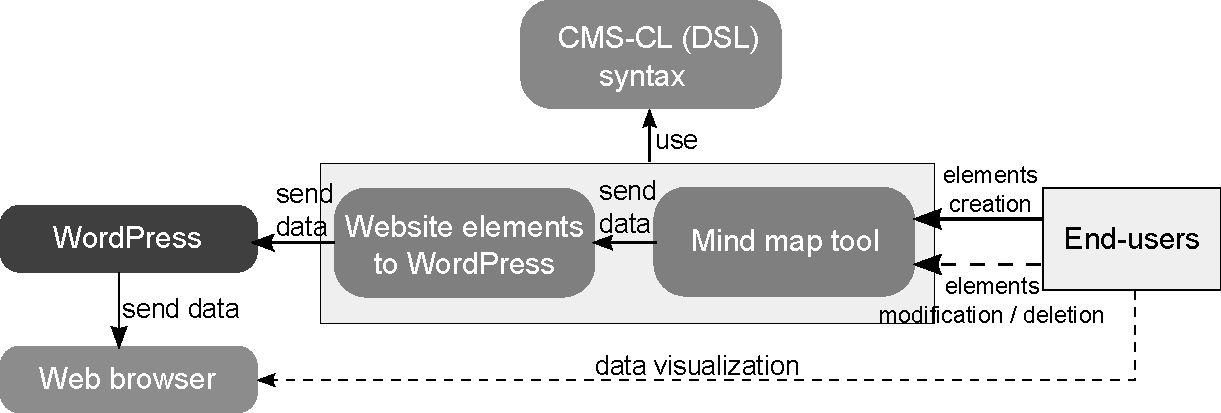
\includegraphics[width=\textwidth]{../resources/pdf/endUsersSimplifiedPresentation.pdf}
		\caption{CMS-CL and mind mapping use}
		\label{CMS-CLMindMappingUse}
	\end{figure}

	As it is presented in Fig.\ref{CMS-CLMindMappingUse}, the use of our defined DSL 	('CMS-CL') with the mind mapping is the following :	
	
	\vspace{0.15em}
	\noindent\textbf{Elements creation.} Using a GUI \footnote{Graphical User Interface}, end users are able to create some website elements.	
	
	\vspace{0.15em}
	\noindent\textbf{Mind-mapping metamodel reduction.} The mind mapping metamodel is reducted to the elements of the CMS-CL metamodel (paragraph \ref{abstractSyntax}). Then, data (elements) are injected into the WordPress platform.	
	
	\vspace{0.15em}
	\noindent\textbf{Data visualization.} After the data injection, it is possible to see the changes on the web site, via a web browser.	
	
	\vspace{0.15em}
	\noindent\textbf{Elements modification and/or deletion.}
	
	\vspace{0.15em}
	\noindent\textit{Deletion:} Users just have to put a delete icon
	(
\includegraphics[scale=0.50]{../resources/png/delete.png}) as described in the section \ref{CMS-CL}, paragraph \ref{concreteSyntax}.
	
	\vspace{0.15em}
	\noindent\textit{Modification:} Users must have to delete first the corresponding element, and recreate a new one with the 					modification. The only exception concerns the 'Website' root node, because it is mandatory : its attribute can be directly modified.